\section{Umsetzung}
\label{sec-5}
\begin{comment}
\fbox{
\parbox{\linewidth}{
	\textit{Ziel des Kapitels:}\\
	Umsetzung erläutern: Wie wurde die Lösungsidee umgesetzt?
}}\\
\end{comment}

Im folgenden soll erläutert werden, wie der zuvor erarbeitete Lösungsansatz umgesetzt wurde. Dazu gibt das Kapitel zunächst einen Überblick über das System und die Architektur der Anwendung. Nach einer kurzen Erläuterung zu ''Screen-Captures'' von der HoloLens folgt eine nähere Betrachtung dessen, wie die Hologramme umgesetzt wurden. Schließlich werden Details zur Interaktion und Performance genannt.

\subsection{Aufbau des Systems}
\label{sec-5-1}
Das System ist als Client-Server-Architektur realisiert, einen Überblick gibt das Schema in Abb. \ref{img:communication-schema}. Ein Server erfasst und verarbeitet die in der Schaltung gemessenen Werte für die Stromstärke. Diese stammen von einem Arduino, der in den Stromkreislauf eingekoppelt ist. Die Applikation auf der HoloLens tritt als Client auf und erfragt die aktuellen Werte vom Server. 
\begin{figure}[H]
	\centering
	\includegraphics[width=1\textwidth]{images/todo.jpg}
	\caption{Schema Kommunikation Schaltung Arduino Server HoloLens}
	\label{img:communication-schema}
\end{figure}

\subsubsection{Client-Server Datenübertragung}
\label{sec-5-1-1}
Die Übertragung der Messwerte vom Arduino zur Anwendung ist so konzipiert, dass Änderungen in Echtzeit übermittelt werden, ohne das unnötiger Netzwerktraffic entsteht. Der Client betreibt ein Polling gegen den Server, der jedoch Antworten solange zurückhält, bis ein neuer, vom vorigen abweichender Wert gemessen wurde. Dieses Verhalten veranschaulicht das Sequenzdiagramm in Abbildung \ref{img:Sequenzdiagramm}. Das Vorgehen führt dazu, dass Änderungen durch den Nutzer am Regler der Spannungsquelle ohne wahrnehmbare Verzögerung auf der HoloLens ankommen.

\vspace{8px}
\begin{center}
	\fbox{
		\parbox{0.9\linewidth}{
			\vspace{4px}
			\textbf{Überblick}
			\begin{itemize}[rightmargin=12px, topsep=-12px]
				\setlength{\itemsep}{-1pt}
				\singlespacing
				\item HoloLens erfragt Daten vom Server über HTTP GET-Requests
				\item Anfragen erfolgen asynchron
				\item Server nimmt den Request entgegen und hält eine Antwort solange zurück, bis ein neuer Wert vom Arduino vorliegt
				\item Dadurch kommen neue Daten sehr schnell bei der HoloLens an, der Nutzer sieht die Änderungen auf der Brille sofort, wenn er Änderungen an der Spannungsquelle vornimmt
				\item So wird zeitliche Einbettung und Kontinuität erreicht
				\item Dabei wird jedoch kein unnötiger Traffic erzeugt
			\end{itemize}
			\vspace{18px}
	}}\\
\end{center}
%\vspace{6px}

\begin{figure}[H]
	\centering
	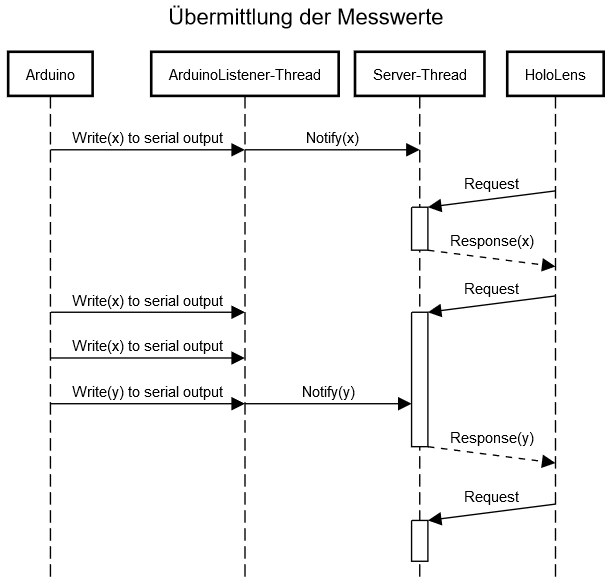
\includegraphics[width=1\textwidth]{images/Sequenzdiagramm.png}
	\caption{Sequenzdiagramm Kommunikation}
	\label{img:Sequenzdiagramm}
\end{figure}

\textit{Server}\\
Der Server besteht aus zwei miteinander kommunizierenden Threads. Ein Thread übernimmt das Lesen und Verarbeiten der Rohdaten, die über die serielle Schnittstelle eintreffen. Bei signifikanten Änderungen wird der zweite Thread mittels einer gemeinsamen, synchronisierten Variablen über die neuen Werte informiert. Dieser beantwortet daraufhin einen ggf. ausstehenden Request vom Client. Ab wann eine Änderung als signifikant gewertet wird, lässt sich über einen Threshold einstellen. Der Server wurde mit Python und der Bibliothek pyserial umgesetzt.\\

\textit{Client}\\
Der Client stellt durch die Nutzung von asynchronen Anfragen sicher, dass die Anfragen nicht blockieren. Unity bietet nur einen Thread, synchrone Anfragen würden daher zu einer Blockierung des Renderprozesses führen und so die Framerate beeinträchtigen. Da die Framerate bei 60 Hz gedeckelt ist und eine Antwort frühestens im nächsten Frame bearbeitet werden kann, beträgt die minimale Antwortzeit ca. 17 ms. Das ist ausreichend, um keine wahrnehmbare Verzögerung aufkommen zu lassen, da die Paketlaufzeit in einem lokalen Netzwerk typischerweise im einstelligen Millisekundenbereich liegt. Eine zusätzliche Wartezeit zwischen Requests kann außerdem eingestellt werden.\\

\subsubsection{Architektur der HoloLens-Anwendung}
\label{sec-5-1-2}
Der Hauptteil des Systems besteht in der auf der HoloLens laufenden Applikation. Die Anwendung basiert auf der Unity Engine und wird als UWP App bereitgestellt. Das Schema in Abb. \ref{img:components-schema} gibt einen Überblick über die verschiedenen Komponenten der Anwendung. Deren Aufgaben sind in der darunter zu findenden Tabelle kurz zusammengefasst.

\begin{figure}[H]
	\centering
	\includegraphics[width=0.7\textwidth]{images/todo.jpg}
	\caption{Schema Komponenten}
	\label{img:components-schema}
\end{figure}


\vspace{8px}
\begin{center}
	\fbox{
		\parbox{0.9\linewidth}{
			\vspace{4px}
			\textbf{Überblick}	
\bgroup
\setlength\extrarowheight{-2pt}
\def\arraystretch{2}
\begin{table}[H]
	\centering
	\begin{tabular}{m{2.5cm}|m{8cm}}
		Komponente & Funktion\\
		\hline
		\hline
		Menu & Hauptmenü, steuert den Ablauf der Anwendung\\
		\hline
		Settings & Lädt und Speichert Einstellungen, bietet Zugang zu den Werten für andere Komponenten und steuert die Einstellungs-Oberfläche\\
		\hline
		Physics & Übernimmt alle physikalischen Berechnungen. Alle relevanten physikalischen Parameter lassen sich konfigurieren.\\
		\hline
		Tracking & Führt durch den Prozess der Positionsbestimmung und setzt den World Anchor\\
		\hline
		Model Anchor & Dient als Anker- und Container-Objekt für die einzelnen Darstellungskomponenten. Dazu gehören: Verdeckungsmodell, Kompass, die Magnetfeldmodelle, die Stromrichtungsindikatoren und das Datenpanel.\\
		\hline
		Webservice & Übernimmt die Kommunikation mit dem Server und gibt erhaltene Daten weiter\\
		\hline
		Interaction & Verarbeitet Input und Ablaufsteuerung, soweit dies nicht an einem konkreten Objekt abgewickelt wird wie z.B. Spracheingabe.\\
	\end{tabular}\caption{\label{tab:components-details} Aufgaben der einzelnen Komponenten}
\end{table}
\egroup
%\vspace{18px}
}}\\
\end{center}
\vspace{6px}

Eine Komponente besteht aus einer Hierarchie von Unity's GameObjects, die mit entsprechenden Skripten versehen sind. Die Komponenten kommunizieren auf unterschiedliche Weise miteinander. Die Behandlung von Events z.B. aufgrund von Nutzereingaben oder neuen Messwerten erfolgt über Callbacks. Manche Komponenten sind auch Singletons, auf die direkt zugegriffen werden kann wie z.B. die Einstellungen.

\subsection{Darstellungen}
\label{sec-5-2}
Nachdem die grundlegende Architektur der vorgestellt wurde folgt nun eine genauere Betrachtung der Umsetzung der Darstellungen. Die Ausführungen werden dabei durch Abbildungen in Form von Screenshots unterstützt. Einen ersten Eindruck vermitteln die Fotos in Abb. \ref{img:HL_SS_Intro}. Damit die von der HoloLens stammenden Bilder richtig interpretiert werden können, sind jedoch einige Vorbemerkungen nötig.

\begin{figure}[h!]
	\centering
	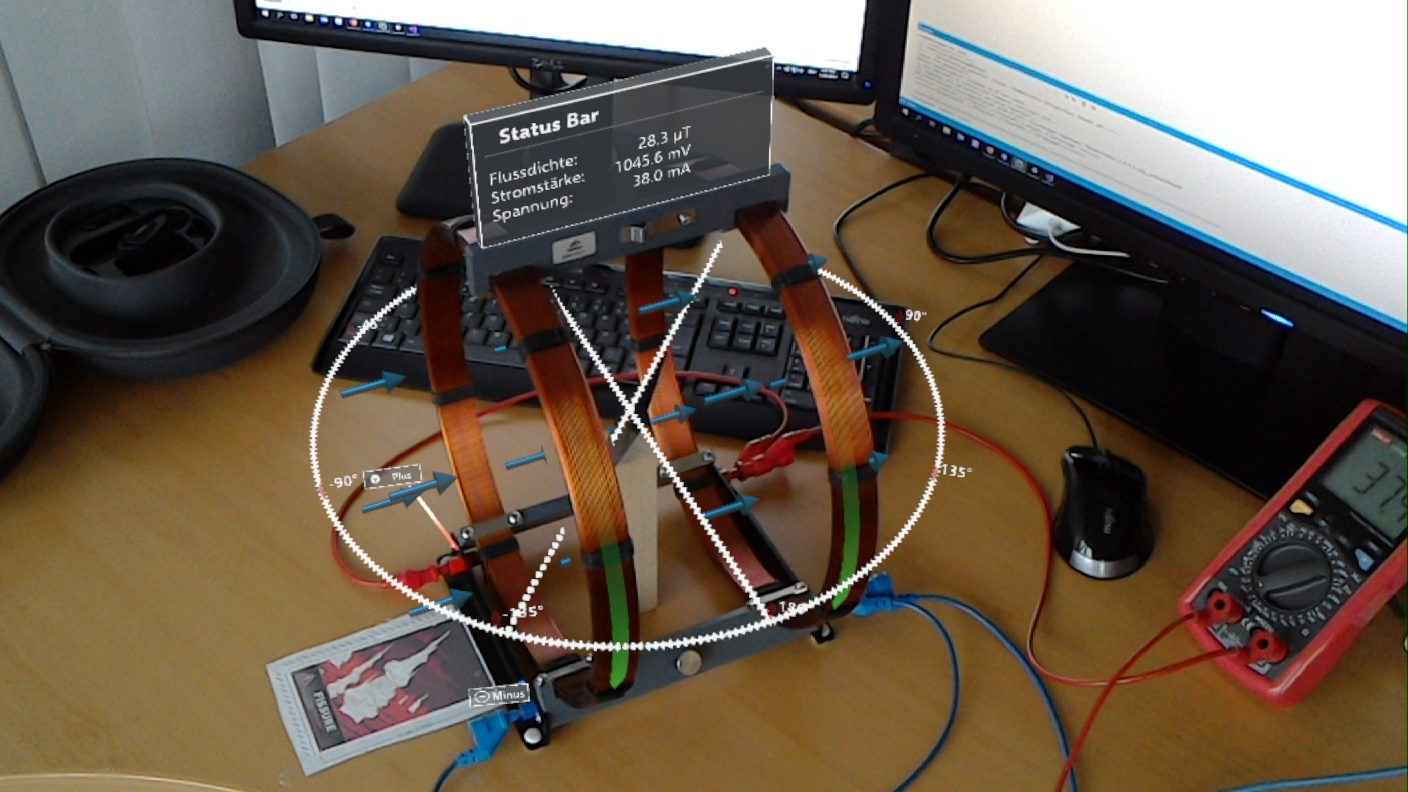
\includegraphics[width=\textwidth]{images/HL_SS1.jpg}

	\vspace{0.25cm}

	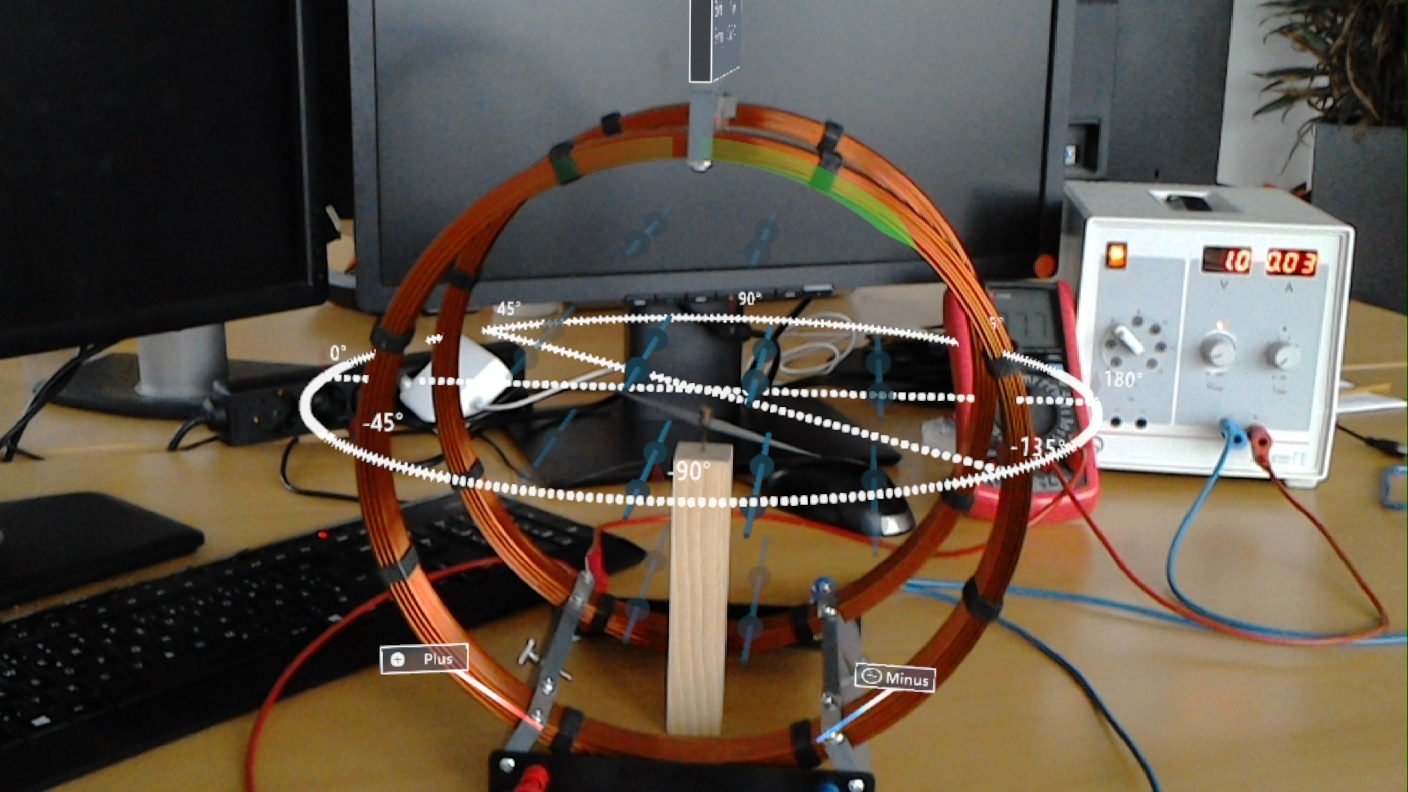
\includegraphics[width=\textwidth]{images/HL_SS2.jpg}
	\caption{Erster Eindruck HoloLens}
	\label{img:HL_SS_Intro}
\end{figure}

\subsubsection{Aufnahmen mit der HoloLens}
\label{sec-5-2-1}
Zunächst ist festzuhalten, dass herkömmliche Bildschirmaufnahmen auf der HoloLens nur eingeschränkt sinnvoll wären. Hier wären nämlich nur die gerenderten Objekte sichtbar, die so auch in einer Entwicklungsumgebung zu sehen sind. Die Nutzererfahrung entsteht jedoch durch das Zusammenspiel mit dem Hintergrund. Deshalb bietet die HoloLens eine angepasste Funktion, um möglichst das abzubilden, was der Nutzer tatsächlich sieht: Das \textit{Mixed Reality Capture (MRC)}.\\

Mit dem Mixed Reality Capture lassen sich Screenshots und Screen-Videos aufnehmen. Dazu nutzt die Brille ihre integrierte Frontkamera und überlagert deren Bild mit dem gerenderten Bild. So lässt sich besser darstellen, was ein Nutzer sieht. Allerdings bringt dieses Vorgehen mehrere Einschränkungen mit sich, durch die die Resultate von den tatsächlich wahrgenommenen Bildern abweichen. Damit die folgenden Bilder richtig eingeordnet werden können, sollen die wichtigsten Faktoren hier genannt werden.

\begin{itemize}
	\singlespacing
	\item Andere Auflösung
	\item Größeres Sichtfeld
	\item Verfälschte Farben und Transparenz
	\item Positionierung
	\item MRC nicht möglich, wenn Kamera durch Anwendung genutzt wird
\end{itemize}

Bei einem MRC-Foto ändert sich die Auflösung von 1268x720 (720p) zu 1408x792. Obwohl die Auflösung steigt ist damit dennoch ein wesentlicher Qualitätsverlust verbunden, da der Betrachter auf der HoloLens zwei HD-Bilder sieht (stereoskopisch), beim Foto aber nur ein Bild erzeugt wird. Außerdem geht die höhere Auflösung des Einzelbildes nicht mit einer höheren Pixeldichte einher, sondern mit einem größeren Sichtfeld. Ein Foto repräsentiert daher nicht die tatsächlichen Begrenzungen des FOV. Dazu kommt die Transparenz von virtuellen Objekten. Diese hängt stark von deren Farbe sowie der Hintergrundhelligkeit ab und entspricht nicht immer der Wahrnehmung des Nutzers. Farbige Objekte erscheinen auf Fotos stets etwas transparent, auch wenn sie den Hintergrund aus Sicht des Nutzers vollständig überdecken. Das trifft z.B. auf die blauen Objekte in den Fotos aus Abb. \ref{img:HL_SS_Intro} zu. Nicht zuletzt ist auch für Fotos die Reduktion der Bildwiederholrate auf 30Hz relevant. Denn dadurch werden die Objekte nicht so gut stabilisiert und es kann zu leichten Verschiebungen auf den Fotos kommen.\\

Darüber hinaus gibt es Faktoren, die durch ein Foto nicht abgedeckt werden können. Dazu gehören die schon erläuterten Eigenheiten der stereoskopischen Wahrnehmung. Auf einem Foto sieht ein Objekt immer scharf aus und es gibt keine Probleme mit der Akkommodation oder Konvergenz, auch wenn ein Nutzer diese möglicherweise erfährt. Außerdem nimmt ein Nutzer die Umgebung anders wahr als auf einem Foto, da das Sichtfeld (auf die Umgebung) kaum eingeschränkt wird und nicht in Farbe und Auflösung begrenzt ist, sondern direkt wahrgenommen wird.\\

Diese Faktoren gilt es bei der Bewertung solcher Bilder zu berücksichtigen. Prinzipiell sind auch Aufnahmen möglich, die näher an die tatsächliche Nutzererfahrung heranreichen. Diese erfordern aber weiteres Equipment, das im Rahmen dieser Arbeit nicht zur Verfügung stand.

\subsubsection{Das Magnetfeld}
\label{sec-5-2-2}
Die Darstellung des Magnetfeldes in Echtzeit erfolgt über 3D-Objekte. Die Geometrie wurde mit Blender erstellt und in Unity importiert. Die Fotos in Abb. \ref{img:mfield-result} zeigen die beiden alternativen Darstellungsmodelle. Darüber hinaus steht eine Visualisierung einer vorberechneten Lösung zur Verfügung, auf die an späterer Stelle genauer eingegangen wird.

\begin{figure}[H]
	\centering
	\includegraphics[width=0.45\textwidth]{images/todo.jpg}
	\hspace{0.05cm}	
	\includegraphics[width=0.45\textwidth]{images/todo.jpg}
	\caption{Links Feldlinien Rechts Vektoren}
	\label{img:mfield-result}
\end{figure}

\vspace{4px}
\begin{center}
	\fbox{
		\parbox{0.9\linewidth}{
			\vspace{4px}
			\textit{Allgemeines}
			\begin{itemize}[rightmargin=12px, topsep=-12px]
				\setlength{\itemsep}{-1pt}
				\singlespacing
				\item Komponenten des Feldes (Erde, Spule) werden mit verschiedenen Farben dargestellt
				\item Feld der Erde ist fest und wird exemplarisch, mittig in der Spule mit der minimal notwendigen Anzahl Elemente gezeigt
				\item Feldlinien / Vektoren als Pfeillinien / Pfeile modelliert
				\item Form wird durch Schattierung betont
				\item Anordnung, Minimum und Maximum (von Abstand bzw. Länge) der Darstellungen sind im Code parametrisiert 
				\item Darstellungsgrenzen über Transparenz (Minimum) und Hardware-Limitierung (Maximum)
			\end{itemize}
			\vspace{18px}
	}}\\
\end{center}
\vspace{6px}

\textit{Visuelle Gestaltung}\\
Die Darstellung des Feldes erfolgt über 3D-Pfeile bzw. -Pfeillinien. Diese werden schattiert, damit die Form und Ausrichtung im Raum besser erkennbar wird. Beide verwenden dafür den gleichen Shader. Die Größe der Objekte wurde anhand von Erfahrungswerten angepasst. Durchmesser und Länge sind vergleichbar mit denen eines Kugelschreibers oder dickeren Stiftes. Als Farben wurden Hellblau und Orange für den Anteil der Spule bzw. der Erde gewählt. Blau wird oft für Magnetfeldlinien verwendet und wird daher auch hier gebraucht. Allerdings wird ein weniger gesättigtes, helleres Blau verwendet, damit die Deckkraft vor helleren Hintergründen nicht verloren geht. Das Orange weißt die selbe Sättigung und Helligkeit auf wie das Blau, damit sich die Objekte nicht in der Transparenz voneinander unterscheiden.\\

\textit{Begrenzung der Darstellung}\\
Die Visualisierung des Feldes erfordert die Festlegung eines darzustellenden Bereiches für die Flussdichte. Ein Intervall lässt sich in der Anwendung frei über die Einstellungen festlegen. Diese Einstellungsmöglichkeit ist für die praktische Nutzung wesentlich, da die gemessene Flussdichte des Erdmagnetfeldes in Abhängigkeit von der Umgebung variieren kann. Voreingestellt ist ein Bereich von $3\mu T$ bis $60\mu T$, die Flussdichte der Erde liegt mit $30 \mu T$ bis $40 \mu T$ im mittleren Bereich dieser Skala. Am unteren Ende des Bereiches werden die Objekte über Transparenz ausgeblendet.\\

Nach oben hin ist keine Darstellung der Begrenzung vorgesehen. Der Bereich sollte so gewählt werden, dass die obere Grenze durch die maximal am Regler einstellbare Stromstärke nicht erreicht werden kann. Somit erfährt der Anwender die Limitierung der Darstellung auf natürliche Weise. Die Konfiguration der Schaltung kann hier über eingebaute Widerstände so an die Spannungsquelle angepasst werden, dass der erzeugte Stromfluss im gewünschten Bereich liegt.\\

\textbf{Feldlinien}\\
Die Feldliniendarstellung ist in Abb. \ref{img:mfield-lines} gesondert abgebildet.
\begin{figure}[H]
	\centering
	\includegraphics[width=0.45\textwidth]{images/todo.jpg}
	\caption{Feldlinien}
	\label{img:mfield-lines}
\end{figure}
\vspace{4px}
\begin{center}
	\fbox{
		\parbox{0.9\linewidth}{
			\vspace{4px}
			\textit{Überblick}
			\begin{itemize}[rightmargin=12px, topsep=-12px]
				\setlength{\itemsep}{-1pt}
				\singlespacing
				\item Pfeillinien repräsentieren Feldlinien über Abstand und Ausrichtung
				\item 4 bis 16 Feldlinien im Gitter angeordnet, orthogonal zur Z-Achse
				\item Anordnung im 3D-Gitter mit konfigurierbaren Parametern (Abstand, Anzahl pro Dimension)
				\item Änderung des Abstandes über Kontraktion zum Mittelpunkt in X-Y-Ebene, Linien werden über Transparenz an der Darstellungsgrenze ein- bzw. ausgeblendet
			\end{itemize}
			\vspace{18px}
	}}\\
\end{center}
\vspace{6px}
\textit{Anordnung}\\
Die Feldlinien der Spule verlaufen orthogonal zur X-Y-Ebene, also in Richtung der Z-Achse. Damit die gewünschten Eigenschaften (Stärke, Homogenität und Richtung) des dreidimensionalen Feldes anhand des Feldlinienmodells erkennbar sind, bedarf es mindestens vier Linien. In einer 2x2 Anordnung um den Mittelpunkt der X-Y-Ebene ist so der Abstand in beiden Dimensionen sichtbar und die Linien sind symmetrisch zur Z-Achse. Anhand der Parallelität lässt sich die Homogenität erkennen und anhand des Abstandes (in der horizontalen oder vertikalen, beide sind gleich groß) die Stärke. Die Flussrichtung ist über eingebaute Pfeilspitzen abgebildet. Als Darstellungsvolumen wurde ein zylindrischer Ausschnitt der Spule gewählt, da diese den Raum besser ausfüllt, als beispielsweise ein kubischer Ausschnitt.\\

\textit{Anzahl}\\
Bei einem festen, für die Darstellungen zur Verfügung stehenden Volumen und kleiner werdenden Abständen müssen zunehmend mehr Linien gezeichnet werden. Zu viele Objekte würden jedoch die Sichtbarkeit anderer Elemente wie Magnetnadel und Kompass beeinträchtigen. Außerdem transportieren zusätzliche Feldlinien keine zusätzlichen Informationen (im Fall eines homogenen Feldes). Allerdings unterstützt die Beobachtung, dass mit zunehmender Flussdichte die Anzahl der Feldlinien steigt, das Verständnis des Feldlinienmodells. Daher wurde für die Umsetzung das Intervall von minimalem und maximalem Abstand so gewählt, dass mindestens 4 und höchstens 16 Linien dargestellt werden. Beim Ein- und Austreten der Objekte in das bzw. aus dem Darstellungsvolumen werden sie kontinuierlich ein bzw. ausgeblendet.\\

\begin{figure}[H]
	\centering
	\includegraphics[width=0.45\textwidth]{images/todo.jpg}
	\caption{Feldlinien Skalierung Abstand}
	\label{img:mfield-lines-scaling}
\end{figure}

\textit{Skalierung}\\
Dabei wurde sich bewusst für die Abbildung der Flussdichte auf den Abstand der Feldlinien entschieden. Das bedeutet, Letzterer ändert sich proportional mit der Flussdichte. Oft wird statt des Abstandes die Anzahl der Feldlinien durch eine Einheitsfläche proportional zur Flussdichte gewählt \cite{Kilian03}. Das bedeutet bei einer symmetrischen Darstellung eines quadratischen Ausschnittes jedoch, dass die Anzahl in diskreten Stufen $n \geq 1$ mit $4^{n}$ steigt. Werden diese Stufen durch eine kontinuierliche Kontraktion der Linien zum Zentrum hin interpoliert, dann skaliert der Abstand $d$ der Feldlinien mit $1/(3n)$. Die Grafik \ref{img:mfield-lines-scaling} illustriert diesen Zusammenhang. Da für den Anwender in erster Linie jedoch der Abstand die sichtbare, sich ändernde Größe ist, könnte dies den falschen Eindruck erwecken, die Flussdichte ändere sich nicht linear mit der Stromstärke. Außerdem werden nur zwei Stufen dargestellt, daher wurde sich für die proportionale Änderung des Abstandes entschieden.\\

\textbf{Vektoren}\\
Die Umsetzung der Vektordarstellung ist in Abb. \ref{img:mfield-vectors} näher zu sehen.
\begin{figure}[H]
	\centering
	\includegraphics[width=0.45\textwidth]{images/todo.jpg}
	\caption{Vektoren}
	\label{img:mfield-vectors}
\end{figure}
\vspace{4px}
\begin{center}
	\fbox{
		\parbox{0.9\linewidth}{
			\vspace{4px}
			\textit{Überblick}
			\begin{itemize}[rightmargin=12px, topsep=-12px]
				\setlength{\itemsep}{-1pt}
				\singlespacing
				\item Pfeile repräsentieren Feldstärkevektor über Länge und Ausrichtung
				\item 8 Pfeile für homogenes Feld, weitere 8 für Andeutung inhomogenes Feld
				\item Anordnung im 3D-Gitter mit konfigurierbaren Parametern (Abstand und Anzahl, jeweils pro Raumrichtung)
				\item Ankerpunkt mittig im Pfeil
			\end{itemize}
			\vspace{18px}
	}}\\
\end{center}
\vspace{6px}

\textit{Anordnung und Anzahl}\\
In der Vektordarstellung werden mindestens acht Vektoren benötigt, damit die zuvor genannten Eigenschaften erkennbar werden. Dabei gelten die gleichen Gründe wie zuvor. Während jedoch eine Feldlinie das Feld in Richtung der Z-Achse kontinuierlich darstellt, sind hier wenigstens zwei Vektoren notwendig. Die Anordnung erfolgt in einem 3D-Gitter, bei dem die Anzahl und die Abstände pro Dimension parametrisiert sind. Auch hier gilt, dass mehr Objekte im homogenen Teil des Feldes keine weiteren Informationen transportieren. Daher wurde in Anbetracht des zur Verfügung stehenden Raumes in die Größe anstelle der Anzahl der Objekte investiert.\\

\textit{Skalierung}\\
Die Flussdichte wird im Fall der Pfeile über deren Länge und Richtung ausgedrückt. Die Form der Objekte soll mit einer sich ändernden Länge nicht verzerrt werden. Eine einfache Skalierung der Pfeillänge würde jedoch dazu führen, dass auch die Pfeilspitze in die Länge gezogen wird. Daher wird die Geometrie zur Laufzeit angepasst und nur ein Teil in der Mitte verändert.\\

\textit{Bezugspunkt}\\
Welcher Punkt dem Vektor als Ankerpunkt dient ist dabei nicht entscheidend, denn ein Pfeil repräsentiert jeden Punkt des homogenen Feldes. Eine explizite Darstellung ist daher nicht erforderlich. Allerdings wird die Verankerung im Mittelpunkt dadurch deutlich, dass die Position bei variierender Länge gleich bleibt.\\

\textit{Inhomogener Anteil}\\
Im Gegensatz zu den Feldlinien ist eine Darstellung des inhomogenen Feldes über Vektoren auch ohne aufwendige Echtzeit-Berechnungen möglich (siehe Kap. \ref{sec-2-2-2}). Die Anwendung nutzt diese Eigenschaft, um in dieser Darstellung auch das inhomogene Feld anzudeuten. Dies geschieht, indem das Raster so gewählt wird, dass vor und hinter der Spule (im Sinne der Z-Achse) jeweils eine Reihe Vektoren positioniert ist. Diese sind hier im Vergleich deutlich kürzer und nicht parallel, sondern nach innen bzw. nach außen gerichtet. So wird erkennbar, dass das Feld hier schwächer und inhomogen ist. Da die Darstellungen erst ab einem minimalen Wert eingeblendet werden, wird der inhomogene Teil nach dem homogenen Teil eingeblendet.\\

 
\textbf{Simulation}\\
Eine Visualisierung der Simulationsdaten ist in Abb. \ref{img:mfield-simulation} näher zu sehen.
\begin{figure}[H]
	\centering
	\includegraphics[width=0.45\textwidth]{images/todo.jpg}
	\caption{Simulation}
	\label{img:mfield-simulation}
\end{figure}
\vspace{4px}
\begin{center}
	\fbox{
		\parbox{0.9\linewidth}{
			\vspace{4px}
			\textit{Überblick}
			\begin{itemize}[rightmargin=12px, topsep=-12px]
				\setlength{\itemsep}{-1pt}
				\singlespacing
				\item Feldlinien vorberechnet mit COMSOL Multiphysics, exportiert als CSV, Import in Unity erfolgt zur Laufzeit
				\item Simulation für einen beliebigen 2D-Querschnitt orthogonal zur X-Y-Ebene, da das Feld symmetrisch zur Z-Achse ist
				\item Anzahl auf 10 Feldlinien festgelegt
				\item Darstellung über 2D-Linien
				\item Rot-Grün Farbskala genutzt
			\end{itemize}
			\vspace{18px}
	}}\\
\end{center}
\vspace{6px}

Die numerische Lösung der Feldgleichungen erfolgte mittels der Simulationssoftware COMSOL Multiphysics. Diese Arbeit konnte hier auf eine bestehende Implementierung einer Helmholtzspule aufbauen. Hier wurden lediglich die folgenden Parameter für die Berechnung der Feldlinien gesetzt:
\begin{itemize}
	\setlength{\itemsep}{-1pt}
	\singlespacing
	\item Anzahl und Anordnung: 10, symmetrisch zur Z-Achse, Abstand entsprechend der Flussdichte
	\item Beschränkung auf die X-Z-Ebene im Radius von 2m um die Spule
	\item Qualitätseinstellungen auf Maximum gesetzt
\end{itemize}
\textit{Export, Import, Datenformat}\\
Das Ergebnis der Simulation ist eine Liste von Datenpunkten der Form \textbf{[}\textit{FeldlinienNr:} Int, \textit{Position:} Vector3, \textit{Betrag der Flussdichte:} float\textbf{]}. Dafür wurde ein CSV-Reader geschrieben, der die Daten zur Laufzeit der Applikation einliest, interpretiert und zum Rendering an GameObjects weitergibt. Folglich ließen sich weitere Simulationen vorberechnen und anzeigen.\\

\textit{Querschnitt}\\
Zunächst ist nur eine Anordnung in der X-Z-Ebene aktiv. Da das Feld aber symmetrisch zur Z-Achse ist, kann mit diesem einen Datensatz bereits jeder Querschnitt durch die Z-Achse dargestellt werden. Bei einer anderen Ausrichtung, z.B. im 45° Winkel, würden jedoch Feldlinien durch den Tisch verlaufen, auf dem die Spule steht.\\

\textit{Rendering}\\
Die Darstellung erfolgt über Unity's Low-Level \textit{Graphics Library (GL)} mittels eines Line-Strips. Dieser ist vergleichbar mit dem von OpenGL, hat aber weniger Funktionen. Insbesondere lässt sich die Dicke der Linien nicht einstellen, sondern ist auf einen Pixel festgelegt. Der sonst in dieser Arbeit für Linien genutzte LineRenderer konnte hier nicht verwendet werden. Denn letzterer ermöglicht für eine Linie nur die Interpolation zwischen maximal 8 Farben. Eine besser Konfigurierbare Darstellung wäre über ein dynamisch generiertes Mesh möglich.\\

\textit{Anzahl und Anordnung}\\
Die Auswahl von 10 Feldlinien erfolgte aus praktischem Ermessen bezüglich der Sichtbarkeit aus 1,5 Metern Entfernung. Dabei wurde bewusst eine gerade Anzahl gewählt. Andernfalls entsteht eine Feldlinie, die genau auf der Z-Achse liegt und nicht geschlossen ist sondern von minus nach plus Unendlich verläuft. Dies wurde aus didaktischen Gründen vermieden.\\

\textit{Farbe}\\
Die Wahl der Farbskala fiel aus mehreren Gründen auf eine Rot-Grün-Skala. Die Linien zeigen die kontinuierliche Änderung der Flussdichte, die durch einen Farbverlauf weiter hervorgehoben werden soll. Dabei kommt es nicht auf das Ablesen der numerischen Werte an, weshalb auch keine Skala mit Farbe und den dazugehörigen Werten angezeigt wird. Es geht viel mehr um das qualitative Verständnis der Darstellung. Mit der gewählten Skala unterscheiden sich die drei wesentlichen Regionen durch ihre Farbe klar voneinander:
\begin{itemize}
	\setlength{\itemsep}{-1pt}
	\singlespacing
	\item Inhomogenes, schwaches Feld außen: Grün
	\item Homogenes, mittel-starkes Feld innen: Gelb
	\item Inhomogenes, starkes Feld unmittelbar am Rand der Spule: Rot
\end{itemize}

Darüber hinaus sprechen technische Gründe für eine solche Farbskala. Damit die Linien in Helligkeit und Transparenz nicht variieren, sollten sich die Farbanteile im RGB-Raum stets zu einem konstanten Wert addieren. Die Rot-Grün-Skala erfüllt diese Eigenschaft, da hier der Blauanteil stets null ist und Rot und Grün über $R = 1 - G$ zusammenhängen. Möglich wären hier auch eine Regenbogenskala, die nicht selten für Magnetfelder angewandt wird\footnote{Vgl. z.B. die Darstellungen in Kap. \ref{sec-2-2} und \ref{sec-2-3}}. Die Skala wird jedoch aufgrund der verzerrten Wahrnehmung nicht empfohlen und wurde hier daher nicht verwendet.

\subsubsection{Stromfluss, Kompass und weitere Darstellungen}
\label{sec-5-2-3}
Nach den Erläuterungen zur Umsetzung der Magnetfelddarstellungen sollen auch die anderen Komponenten kurz beleuchtet werden.\\

\textbf{Stromfluss}
\vspace{4px}
\begin{center}
	\fbox{
		\parbox{0.9\linewidth}{
			\vspace{4px}
			\textit{Richtungsindikatoren}
			\begin{itemize}[rightmargin=12px, topsep=-12px]
				\setlength{\itemsep}{-1pt}
				\singlespacing
				\item Darstellung über breite 2D-Linien mit Unity's \textit{LineRenderer}, die an einem Ende zu einer Pfeilspitze zusammenlaufen
				\item Liegen direkt auf der Spule auf und sind fest, richten sich also nicht zur Kamera aus
				\item Es werden stets nur Pfeile angezeigt, die der Nutzer gerade sehen kann
				\item Dazwischen werden die Pfeile kontinuierlich ein- bzw. ausgeblendet
			\end{itemize}
			\vspace{18px}
	}}\\
\end{center}
\vspace{6px}

Die Indikatoren werden dynamisch über ein Skript erzeugt und gesteuert. Hier können Parameter wie Richtung, Position, Radius und Bogenlänge festgelegt werden. Die Breite der Linien wurde auf 1cm gesetzt. Die Größe ist für die gewünschte Entfernung ausreichend und übersteigt die Dicke der Spulen nicht. Indem die Darstellung sich der Betrachtungsposition kontinuierlich anpasst wird der Nutzer zusätzlich in die Anwendung einbezogen.\\

\textit{Strom-Labels}\\
Die Richtungspfeile werden durch die Information unterstützt, wie die Spule in die Schaltung eingebunden ist. Dazu werden die Anschlüsse mit Annotationen versehen.
\begin{itemize}
	\setlength{\itemsep}{-1pt}
	\singlespacing
	\item Plus- und Minus-Kennzeichner über Tooltip-Elemente des MRTK umgesetzt
	\item Verbindungslinien farblich an die Farbe der Verbindungsstücke angepasst
	\item Tooltips um Plus- und Minus-Icons ergänzt
\end{itemize}

Hier konnte auf ein vorgefertigtes Tooltip-Objekt des MRTK zurückgegriffen werden. Diese wurden um die entsprechenden Farben und Icons ergänzt. Die Icons basieren auf freien Icon-Packeten \footnote{https://icons8.com}, wurden jedoch angepasst. Da schwarze Strukturen vor transparentem Grund auf der HoloLens so nicht zu sehen sind, wurde der Hintergrund bzw. die Icon-Struktur zu weiß geändert.\\

\textbf{Kompass}\\
Der Kompass besteht aus einer virtuellen Skala und einer realen Magnetnadel in der Mitte. Die verschiedenen Linien wurden als gestrichelte, leicht transparente 2D-Linien umgesetzt.
\vspace{4px}
\begin{center}
	\fbox{
		\parbox{0.9\linewidth}{
			\vspace{4px}
			\textit{Linien}
			\begin{itemize}[rightmargin=12px, topsep=-12px]
				\setlength{\itemsep}{-1pt}
				\singlespacing
				\item Darstellungen über gestrichelte 2D-Linien mit Unity's LineRenderer
				\item Gestrichelte Linie durch Textur mit weißem Kreis und transparentem Hintergrund, Skalierung auf die Länge der Linie mit Tiling
				\item Billboard-Verhalten für Sichtbarkeit aus unterschiedlichen Winkeln
				\item Grau als Farbe genutzt, leicht transparent, virtueller Kompass jedoch etwas heller und daher präsenter gestaltet
			\end{itemize}
			\vspace{18px}
	}}\\
\end{center}
\vspace{6px}

Der Kompass liegt horizontal in einer Ebene durch den Spulenmittelpunkt. Die ringförmige Skala wurde mit einem Radius von 20 cm sehr eng um die Spulen herum gelegt, damit wenig zusätzliches Sichtfeld benötigt wird. Denn je größer der Raduis, desto eher wird das Element durch die Sichtfeldbegrenzung abgeschnitten. Neben den festen Gradzahlen im Abstand von 45° wird hier auch die theoretisch berechnete Gradzahl am Ende der zugehörigen Linie angezeigt.\\

Als Farbe wurde Grau gewählt, damit die Linien neutral und weniger dominant wirken. Dem dient auch die Wahl von gestrichelten anstelle durchgezogener Linien. Gleichzeitig wurde die zuvor dunkle Magnetnadel hell angemalt, damit sie zwischen den virtuellen Objekten besser zu sehen ist.\\

In dieser Umsetzung wird zunächst keine Verdeckung durch die Magnetnadel berechnet. Diese ließe sich anhand der theoretischen Auslenkung berechnen. Allerdings unterliegt die reale Nadel Trägheit und Reibung, die in der Berechnung nicht berücksichtigt werden. Außerdem ist sie sehr schmal (etwa 5 mm breit), weshalb Abweichungen zwischen realem und virtuellem Modell stärker ins Gewicht fallen, als bei größeren Objekten. Daher verzichtet diese Lösung darauf, was sich jedoch negativ auf die Immersion des Anwenders auswirkt.\\

\textbf{Datenpanel und weitere Informationen}\\
Nicht zuletzt wurden von den als optional eingestuften Informationen die ausgewählt, die im Zusammenhang mit den Echtzeitdaten stehen, und für diese eine textuelle Darstellung umgesetzt.
\vspace{4px}
\begin{center}
	\fbox{
		\parbox{0.9\linewidth}{
			\vspace{4px}
			\textit{Status Bar}
			\begin{itemize}[rightmargin=12px, topsep=-12px]
				\setlength{\itemsep}{-1pt}
				\singlespacing
				\item Listet gemessene und berechnete Echtzeitwerte auf: Stromstärke, Spannung, Flussdichte
				\item 4 Replikas, Platzierung an unteren Balken zwischen den Spulen
				\item Sichtbarkeit analog zu Strom-Pfeilen
				\item Dunkelgrauer Hintergrund für bessere Lesbarkeit
			\end{itemize}
			\vspace{18px}
	}}\\
\end{center}
\vspace{6px}
Das Datenpanel listet die numerischen Werte für die genannten Größen zusammen mit ihren Einheiten auf. Der Hintergrund orientiert sich an dem des vorgefertigten Tooltips und wird einheitlich für alle Texte (abgesehen von den Buttons) verwendet. Die Objekte sind schräg gestellt (ca. 35°), so dass sie aus diesem typischen Winkel gut zu lesen sind.\\

Durch ihre Platzierung unmittelbar über dem Untergrund würden Drop Shadows das Präsenzgefühl stärken. Diese lassen sich hier jedoch nicht direkt umsetzen, denn der Untergrund ist real und kann durch die HoloLens nicht weiter verdunkelt werden. Eine mögliche Lösung bestünde darin, die Schatten zu erzeugen, indem der Untergrund außerhalb des Schattens zusätzlich erhellt wird. Allerdings müssten hier wiederum die Schatten der realen Objekte mit einbezogen werden. Daher nimmt diese Lösung die fehlenden Schatten in Kauf.\\

Die weiteren, optional einblendbaren Informationen wie Spulenabstand oder Windungszahl wurden aus zeitlichen Gründen nicht umgesetzt, da hier eine weitere Interaktionsmöglichkeit einzurichten wäre, um die Elemente ein- und auszublenden.

\subsubsection{Weitere technische Komponenten}
\label{sec-5-2-4}
Die Implementierung der Darstellungen wird begleitet von weiteren technischen Lösungen, auf die dieser Abschnitt näher eingehen soll.
\vspace{8px}
\begin{center}
	\fbox{
		\parbox{0.9\linewidth}{
			\vspace{4px}
			\textit{Überblick}
			\begin{itemize}[rightmargin=12px, topsep=-12px]
				\setlength{\itemsep}{-1pt}
				\singlespacing
				\item Spule maßstabsgetreu für Verdeckungsberechnung modelliert mit ca. 2mm größerer Ausdehnung, Rendering ausschließlich in den Z-Puffer
				\item Near Plane Fading verbirgt Objekte, die eine minimale Distanz zur Kamera unterschreiten
				\item Progress Indikator informiert über Zustand länger laufender Vorgänge, z.B. Ladevorgang der Simulationsdaten oder Einlesen des Markers
				\item Kantenglättung durch 2x MSAA
			\end{itemize}
			\vspace{18px}
	}}\\
\end{center}
\vspace{6px}

\textit{Occlusion Berechnung}\\
Für die Verdeckungsberechnung wurde die Spule anhand gemessener Größen in Blender modelliert. Das Spatial Mapping der HoloLens ist hier zu ungenau, um eine glaubwürdige Verdeckung zu ermöglichen. Eine Gegenüberstellung des durch die HoloLens aufgenommenen Spatial Mappings mit der modellierten Geometrie ist in Abb. \ref{img:mesh-vs-model} zu sehen.
\begin{figure}[H]
	\centering
	\includegraphics[width=0.45\textwidth]{images/todo.jpg}
	\hspace{0.05cm}	
	\includegraphics[width=0.45\textwidth]{images/todo.jpg}
	\caption{HoloLens Mesh vs. Modell}
	\label{img:mesh-vs-model}
\end{figure}
Die Geometrie wird ausschließlich in den Tiefenpuffer gerendert\footnote{Der entsprechende Shader ist nur wenige Zeilen lang und findet sich in verschiedenen Varianten im Internet. Dieser orientiert sich an http://wiki.unity3d.com/index.php/DepthMask}. Das vermeidet überflüssige Draw Calls und folgt der Empfehlung der Dokumentation. Damit virtuelle Objekte aber auch dann noch verdeckt bleiben, wenn reale Objekte nah kommen, muss das Near Clipping Plane sehr nah am Kameraursprung liegen. Andernfalls würden weiter entfernte, virtuelle Objekte plötzlich doch vor realen Objekten angezeigt werden, sobald letztere zu nah sind und das Clipping die für die Verdeckung eingesetzten Objekte vom Rendering ausschließt. Das stellt bei dieser Lösung aber kein Problem dar, weil zu nahe, virtuelle Objekte ohnehin über ein eigenes Verhalten ausgeblendet werden, das nicht auf die Clippingebene aufbaut.\\


\textit{Near Plane Fading}\\
Anstelle auf Basis der Clippingebene werden zu nahe Objekte über Skripte bzw. Shader kontinuierlich ausgeblendet. Dieses Verhalten ist für den Nutzer angenehmer als ein plötzliches Aufpoppen bzw. Verschwinden von Objekten in unmittelbarer Nähe.\\

Der für die meisten Objekte genutzt MRTK Standard Shader bietet bereits einen konfigurierbaren Bereich, über den Objekte ausgeblendet werden. Für andere Elemente wird die Transparenz über ein Skript geregelt. Hier werden für Anfang und Ende des Bereiches, über den zur Transparenz übergegangen wird, die empfohlenen Werte von 85cm und 50cm genutzt. Lediglich die Linien des Kompasses werden 10 cm ''später'' ausgeblendet, damit die Ausrichtung der Nadel entlang der Linien auch aus geringerem Abstand und damit etwas besser erfasst werden kann. Insgesamt ergibt sich die Transparenz (Alpha-Wert) eines Objektes dann aus dem Minimum der Werte durch die verschiedenen Effekte.\\

Diese Lösung geht jedoch zu Lasten der Performance, denn für die Transparenz werden alle betroffenen Objekte von hinten nach vorne (aus Sicht der Kamera) gerendert. Auch Pixel, die durch weiter vorne gelegene Objekte eingenommen werden, müssen mehrfach gezeichnet werden, da die dichteren Objekte ggf. transparent sind und durch die Farbe anderer Objekte beeinflusst werden. Dieser sogenannte Overdraw nimmt zusätzliche Rechenzeit in Anspruch. Eine Alternative bestünde darin, Objekte schwarz anstatt transparent werden zu lassen. Auf der HoloLens macht dies optisch zunächst keinen Unterschied, da Schwarz auf der Brille nicht dargestellt wird. Allerdings bliebe so die Verdeckung durch bereits verschwundenen Objekte bestehen, was zu Irritationen führen würde.\\

\textit{Progress Indikator}\\
Um den Anwender über länger laufende Prozesse zu informieren, kommt eine Fortschrittsanzeige zum Einsatz. Hier kann auf den aus Mircosoft Windows bekannten Indikator zurückgegriffen werden, den das MRTK als vorgefertigtes Objekt anbietet. Das Mixed Reality Capture in Abb. \ref{img:pi-and-tracking} zeigt diesen beim Start der Anwendung.\\

\begin{figure}[H]
	\centering
	\includegraphics[width=0.45\textwidth]{images/todo.jpg}
	\hspace{0.05cm}	
	\includegraphics[width=0.45\textwidth]{images/todo.jpg}
	\caption{Progress Indikator Laden und Tracking}
	\label{img:pi-and-tracking}
\end{figure}

Für die Kommunikation mit dem Nutzer ist bei dieser Anwendung vor allem wichtig, was das System tut. Längere Ladezeiten o.Ä. treten hier nicht auf, daher wird lediglich das Text-Element des Indikators verwendet, von der prozentualen Anzeige wird nicht Gebrauch gemacht. Komponenten, die den Indikator nutzen, stellen jedoch stets sicher, dass eine Nachricht lange genug sichtbar ist, um gelesen werden zu können. Länger laufende Operationen sind stets asynchron umgesetzt, die pro Frame nur einen Teil der Arbeit erledigen und so den Renderprozess nicht blockieren.\\

\textit{Kantenglättung}\\
Bei Darstellungen auf der HoloLens fällt der Kantenglättung eine besondere Bedeutung zu. Im Gegensatz zu anderen Anwendungen, bei denen denen der Nutzer die Kamera über herkömmliche Eingabegeräte steuert, ist bei der Brille die Kamera an die Kopfbewegungen des Trägers gebunden. Die Displays folgen daher den ständigen, feinen Vibrationen des Kopfes, die Kamera steht also nie still. Deshalb können Treppeneffekte an Kanten besonders auffällig und störend wirken, da das resultierende Kantenflimmern stetig präsent ist. Allerdings sind Anti-Aliasing-Verfahren wie z.B. Multi Sampled Anti Aliasing oft mit erheblichem Rechenaufwand verbunden.\\ % Die Dokumentation der HoloLens empfiehlt daher, auf den Einsatz solcher Verfahren zu verzichten.\\

Für die gewählte Visualisierung der Simulationsdaten über Linien ist eine Form des Anti-Aliasing jedoch unerlässlich. Andernfalls würde hier die gesamte Darstellung flimmern. Deshalb wurde sich hier für den Einsatz von zweifachem Multi-Sampled Anti-Aliasing (MSAA) entschieden. Das Verfahren wird durch Unity standardmäßig unterstützt und kann ohne weitere Maßnahmen für die Kamera aktiviert werden. Die Dokumentation rät zwar im Rahmen der Hinweise zu ressourcenschonenden Maßnahmen vom Einsatz solcher Verfahren ab. Da die Anwendung jedoch sonst keine besonders aufwendigen Berechnungen ausführen muss und der Qualitätsgewinn deutlich wahrnehmbar ist, wird MSAA dennoch verwendet.


% Einzig das Starten und Stoppen des Trackingframeworks 
\begin{comment}
\textit{Künstliche Beleuchtung}\\
Beleuchtung bildet grob erwartete Lichtverhältnisse nach, keine Schatten\\
\begin{itemize}
\item Virtuelle Beleuchtung von Oben bildet echte Lichtverhältnisse grob nach
\item Unterstützt die Einbettung der 3D Objekte im Raum
\end{itemize}
\end{comment}

\subsection{Rahmen der Anwendung}
\vspace{8px}
\begin{center}
	\fbox{
		\parbox{0.9\linewidth}{
			\vspace{4px}
			\textit{Überblick}
			\begin{itemize}[rightmargin=12px, topsep=-12px]
				\setlength{\itemsep}{-1pt}
				\singlespacing
				\item Tracking mit Vuforia, nur zum Erkennen des Markers aktiv
				\item Einstellungen werden als JSON-Datei im AppData Verzeichnis gespeichert
				\item Menü übernimmt Steuerung der einzelnen Vorgänge, jederzeit aufrufbar
				\item Startvorgang mit Intro-Sequenz lädt Daten und Einstellungen und initialisiert Komponenten
			\end{itemize}
			\vspace{18px}
	}}\\
\end{center}
\vspace{6px}


\textit{Tracking}\\
Für das Erkennen der Markerposition kommt das Tracking Framework Vuforia zum Einsatz. Ein optischer Marker wird vor der Spule auf dem Untergrund platziert. Dieser wird dann über die Frontkamera der HoloLens durch das Framework erkannt und die Position und Ausrichtung bestimmt. Die Modelle werden entsprechend positioniert und ein World Anchor gesetzt. Damit ist die Positionierung abgeschlossen und der Marker kann entfernt werden. Da Vuforia nur während dieser Sequenz aktiviert ist, werden für den Rest der Anwendung Hardwareressourcen frei.\\

Dieser Vorgang lässt sich über das Menü jederzeit neu anstoßen und die einzelnen Schritte werden über den Progress Indikator dem Nutzer kommuniziert. Die Steuerung des Prozesses erfolgt durch den \textit{Tracking Manager}. Dieser startet und stoppt das Framework, reagiert auf Änderungen im Tracking und informiert den Anwender über den Fortschritt. Der Screenshot\footnote{Wie in Kap. \ref{sec-5-2-1} festgehalten sind während des Trackings keine Aufnahmen mit der HoloLens möglich, da die Kamera von Vuforia in Anspruch genommen wird.\nopagebreak} in Abb. \ref{img:pi-and-tracking} zeigt eine solche Nachricht.\\

\textit{Einstellungen}\\
Die Einstellungen sind über ein dem Daten-Panel ähnliches Objekt realisiert, das in Abb. \ref{img:menu-and-settings} zu sehen ist. Ein Klick auf eines der Input-Felder ruft die virtuelle Tastatur hervor, beide werden durch das MRTK bereitgestellt und wurden hier für numerische Eingaben konfiguriert. Die Werte werden als JSON formatiert und in das AppData-Verzeichnis der Anwendung gespeichert. Damit stehen sie auch nach einem Neustart oder Update der App noch zur Verfügung. Die Applikation sucht beim Start automatisch nach gespeicherten Einstellungen und lädt entweder diese oder die Default-Werte. Andere Komponenten werden durch ein Event über sich ändernde Einstellungen benachrichtigt und passen sich entsprechend an.\\

\begin{figure}[H]
	\centering
	\includegraphics[width=0.45\textwidth]{images/todo.jpg}
	\hspace{0.05cm}	
	\includegraphics[width=0.45\textwidth]{images/todo.jpg}
	\caption{Einstellungen und Menü}
	\label{img:menu-and-settings}
\end{figure}

\textit{Menü}\\
Die Umsetzung des Menüs ist in Abb. \ref{img:menu-and-settings} abgebildet. Die Form der Buttons wurde so angepasst, dass die Labels und Icons problemlos darauf Platz finden. Bei den Icons wurde auf Standard-Elemente aus dem MRTK zurückgegriffen. Das Menü wird über den \textit{MenuController} gesteuert, von dem aus alle weiteren Vorgänge gestartet werden. Dieser aktiviert auch den Cursor, der zur Nutzung von Menu und EInstellungen dient.\\

\textit{Intro-Sequenz}\\
Es wurde eine Startsequenz entwickelt, die Aufgaben wie das Laden von Daten und Einstellungen und die Initialisierung der einzelnen Komponenten übernimmt. Hier wird ein Logo in Form eines größeren Schriftzuges und dazu der Progress Indikator angezeigt. Letzterer informiert über den Zustand des Ladevorgangs. Während des Vorgangs werden insbesondere die Einstellungen und  Simulationsdaten geladen.\\

Diese Umsetzung erlaubt die notwendigen Ladevorgänge und ist für den Nutzer nachvollziehbar. Außerdem gibt das letzterem einige Sekunden Zeit, um sich auf die Anwendung einzustellen, bevor das Menü erscheint und eine Aktion vom Anwender verlangt.


\subsection{Interaktion}
Die Interaktion erfolgt, wie in Kap. \ref{sec-4-4} beschrieben, durch Klicks. Sprachbefehle wurden aus Zeitgründen nur für Debugging-Funktionen implementiert. 
Während des Hauptteils der Anwendung belaufen sich die möglichen Aktionen auf:

\begin{itemize}
	\setlength{\itemsep}{-1pt}
	\singlespacing
	\item Klick: Wechsel zwischen den beiden Echtzeitdarstellungen
	\item Doppelklick: Wechsel zwischen Simulations- und Echtzeitdarstellungen
	\item Hold-Klick: Aufrufen des Hauptmenüs
\end{itemize}

Für die letzteren beiden wurden entsprechende Skripte geschrieben, die diese Gesten erkennen. Zwar erkennt das MRTK bereits eine Hold-Geste, allerdings kann hier der Nutzer beliebig lange gedrückt halten und erst beim Loslassen feuert das entsprechende Event. Zum Aufrufen des Menüs ist jedoch ein Verhalten wünschenswert, bei dem nach kurzem Gedrückt-Halten das Menü erscheint. Daher wurde hier eine eigene Lösung entwickelt.\\

Jeder Klick wird durch einen Klick-Sound begleitet, der als Feedback dient. Ist der Cursor aktiv, bietet dieser auch ein visuelles Feedback. Als Klick-Sound wurde ein Standard-Sound des MRTK verwendet, der auch von den Buttons genutzt wird.

\subsection{Performance}
Zuletzt sollen einige Maßnahmen genannt werden, die zu einem geringeren Ressourcenverbrauch der Applikation beitragen. Zunächst ist festzuhalten, dass die durch das MRTK voreingestellten Qualitätseinstellungen genutzt wurden. Einzige Ausnahme stellt hier die Kantenglättung dar. Darüber hinaus wurden die folgenden Einstellungen angewandt:

\begin{itemize}
	\setlength{\itemsep}{-1pt}
	\singlespacing
	\item Single Pass Instanced Rendering
	\item Größe des Tiefenpuffers auf 16-Bit gesetzt (Minimum)
	\item Vuforia nur für den Vorgang der Positionsbestimmung aktiv
	\item Physics Enginge deaktiviert
	\item Frustum Culling aktiviert
	\item Occlusion Mesh wird ausschließlich in Z-Puffer gerendert
	\item Unsichtbare (vollst. transparente) Objekte werden meist deaktiviert
\end{itemize}

Diese Maßnahmen basieren vorrangig auf den Empfehlungen zur Performance in der Dokumentation.